% Churn prediction model (~1 minute, 4 frames). Figures: report Chapters 5-6.
\section{Churn Prediction Model}

% ---- Step card for the preparation pipeline: fixed size, top-aligned ----
\newcommand{\prepstep}[4]{%
  \begin{tikzpicture}[baseline=(card.north)]
    \node (card) [rounded corners=6pt, fill=cardgray, inner sep=8pt] {%
      \parbox[t][3.7cm][t]{2.7cm}{\raggedright
        \cardbadge{#1}\\[6pt]
        {\bfseries\small\color{hustcrimson} #2}\\[2pt]
        {\bfseries\LARGE #3}\\[4pt]
        {\footnotesize\color{inkgray} #4\par}}%
    };
  \end{tikzpicture}%
}
\newcommand{\steparrow}{\raisebox{-2.2cm}{\color{hustcrimson}\Large$\rightarrow$}}

\begin{frame}{From transactions to a weekly modeling table}{One row per customer per Monday, built only from information up to that date}
  \vspace{0.4cm}
  \centering
  \prepstep{1}{Clean}{72.8\%}{of raw rows kept}%
  \hfill\steparrow\hfill
  \prepstep{2}{Weekly population}{$\sim$2.6k}{active customers per week}%
  \hfill\steparrow\hfill
  \prepstep{3}{Label}{48.0\%}{churn: no purchase in the next 90 days}%
  \hfill\steparrow\hfill
  \prepstep{4}{Features}{11}{RFM\\ Order value\\ Purchase timing\\ Products\\ Cancellations}

  \vspace{0.5cm}
  {\scriptsize\color{inkgray} Active $=$ bought before and last purchase $\leq$ 136 days ago (P90 repurchase gap).}
\end{frame}

\begin{frame}{Leakage-safe temporal split}{Chronological periods, with a 90-day embargo so no label window reaches the next period}
  \centering
  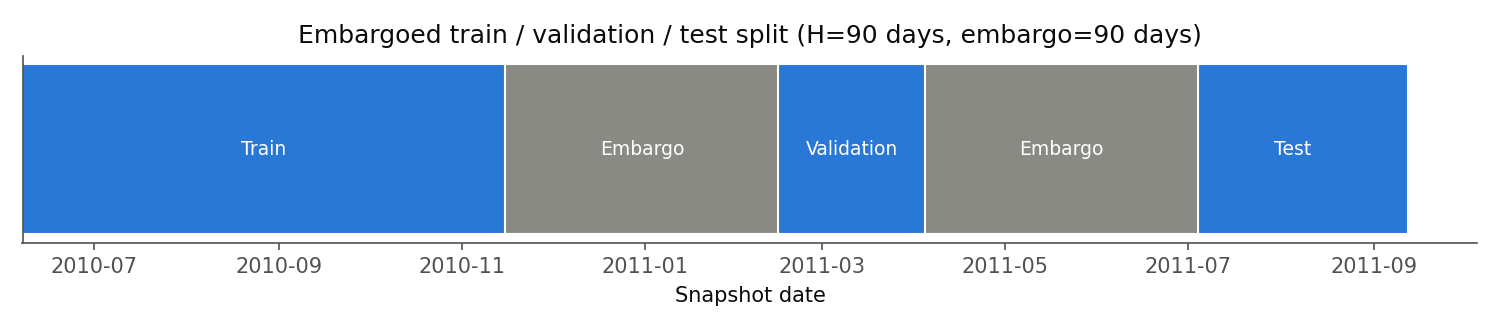
\includegraphics[width=0.92\textwidth]{figures/split_timeline.png}

  \vspace{0.2cm}
  \small
  \begin{tabular}{@{}llrrr@{}}
    \toprule
    Period & Snapshot dates & Weeks & Rows & Churn rate \\
    \midrule
    Train & Jun -- Nov 2010 & 24 & 61,415 & 43.0\% \\
    Validation & Feb -- Apr 2011 & 8 & 21,514 & 52.9\% \\
    Test & Jul -- Sep 2011 & 10 & 24,252 & 40.1\% \\
    \bottomrule
  \end{tabular}

  \vspace{0.15cm}
  {\scriptsize\color{inkgray} A 6-month warm-up precedes the first snapshot so every customer has some history. The churn rate moves with the season between periods.}
\end{frame}

\begin{frame}{Model selection and tuning on validation}{Final: Logistic Regression $\cdot$ Extended features (8) $\cdot$ $C = 0.01$ $\cdot$ refit on train $+$ validation}
  \vspace{0.2cm}
  \begin{columns}[t]
    \column{.58\textwidth}
    \footnotesize
    \begin{tabular}[t]{@{}llccc@{}}
      \toprule
      Step & Candidate & AUC & Brier & \\
      \midrule
      Baselines & Random & 0.495 & -- & \\
       & Recency rule & 0.673 & -- & \\
      \midrule
      Training rows & A -- Episode sample & 0.774 & 0.226 & \\
       & B -- All weekly, weighted $1/n_i$ & \textbf{0.781} & \textbf{0.214} & \checkmark \\
      \midrule
      Features & RFM (3) & 0.778 & 0.218 & \\
       & Extended (8) & \textbf{0.781} & \textbf{0.214} & \checkmark \\
       & Full (11) & 0.781 & 0.214 & \\
      \midrule
      Algorithm & Logistic Regression & \textbf{0.781} & \textbf{0.214} & \checkmark \\
       & Random Forest & 0.770 & 0.222 & \\
       & XGBoost & 0.756 & 0.238 & \\
      \bottomrule
    \end{tabular}
    \column{.36\textwidth}
    \footnotesize
    \begin{tabular}[t]{@{}lccc@{}}
      \toprule
      $C$ (L2) & AUC & Brier & Tied? \\
      \midrule
      0.001 & 0.775 & 0.213 & no \\
      0.003 & 0.777 & 0.210 & no \\
      \textbf{0.01} & \textbf{0.780} & \textbf{0.210} & \checkmark \\
      0.1 & 0.781 & 0.213 & yes \\
      100 & 0.781 & 0.214 & best \\
      \bottomrule
    \end{tabular}
  \end{columns}
\end{frame}

\begin{frame}{Model evaluation on test}{Scored once on the 10 test weeks with calibrated probabilities}
  \centering
  \stattile{0.744--0.773}{AUC per week}\hfill
  \stattile{0.194}{Brier score}\hfill
  \stattile{0.110}{HHI of 10 risk bands}\hfill
  \stattile{0.08 $\rightarrow$ 0.14}{CSI vs.\ validation}

  \vspace{0.25cm}
  \begin{columns}[t]
    \column{.49\textwidth}
    \centering
    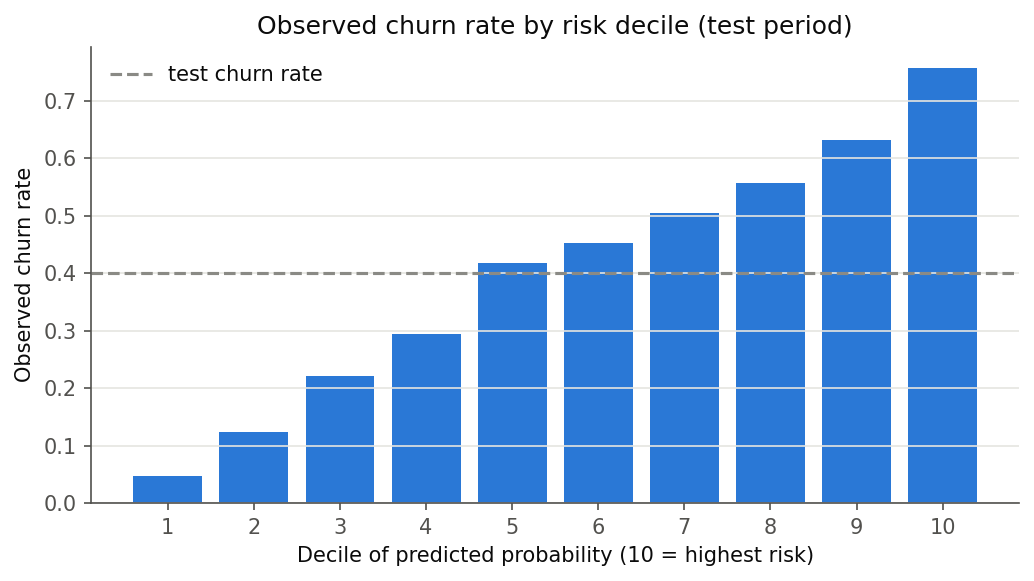
\includegraphics[width=\textwidth, height=4.4cm, keepaspectratio]{figures/gain_by_decile.png}
    \column{.49\textwidth}
    \centering
    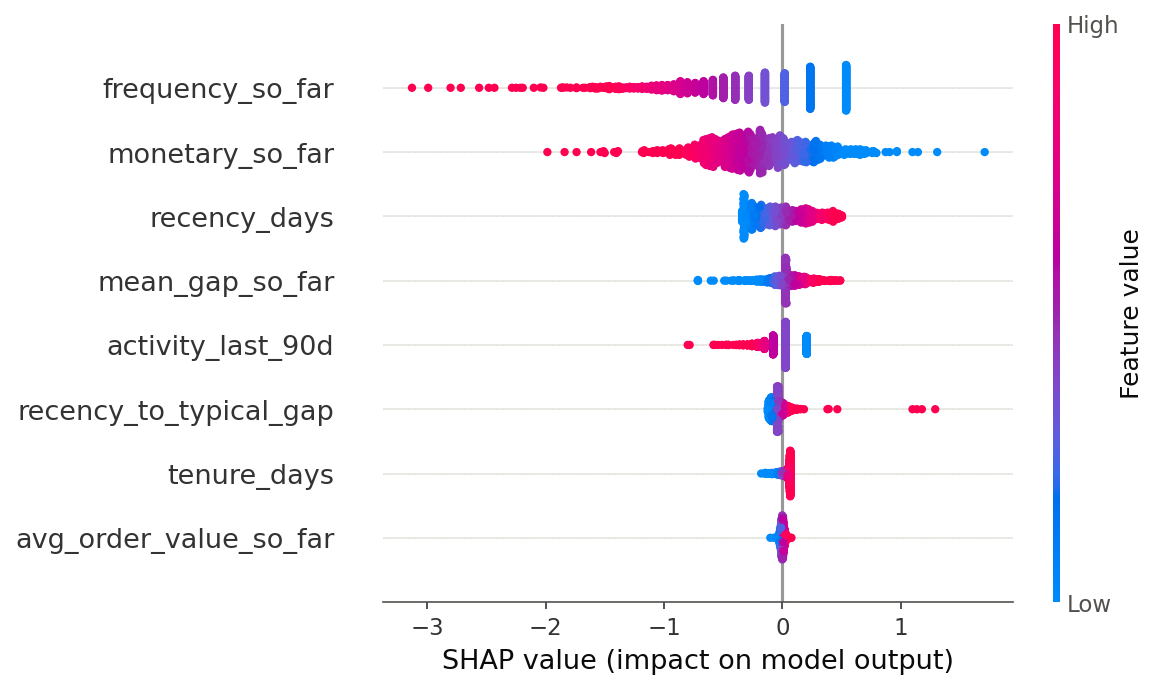
\includegraphics[width=\textwidth, height=4.4cm, keepaspectratio]{figures/shap_summary.png}
  \end{columns}
\end{frame}
